\section {User Interfaces Intro}

The term Z-Way refers to a software architecture for a Z-Wave Network Controller that consists of several parts.

\begin{itemize}

\item {\bf The Z-Way server:} This software runs on top of your operating system or inside your appliance. It handles
all Z-Wave network related functions and has a built-in web server to support User Interfaces
\item {\bf The Demo User Interface:} This is one of the User Interfaces. It is not optimized in terms of design and fashion but
it will show all functions of the Z-Wave network and the Z-Wave devices and give users access to all data 
related to the management of a Z-Wave network and to the operation of Z-Wave devices in this network.
\item {\bf Other User Interfaces:} Z-Way provides several other user interfaces that offer a subset of the Demo User 
Interfaces functionality but may enhance them with own logic.
\end{itemize}

The next chapters describe the purpose and the use of the Z-Way server and the Demo User Interface. This means
that the following four areas are \underline{not scope of this manual}:

\begin{itemize}
\item {\bf Z-Way development:} There is a separate manual {\bf Z-Way Developers Manual} with instructions how to 
develop your own User Interface using the Z-Way Server. You can download this manual e.g. from the Z-Wave.Me 
Home Page www.z-wave.me.
\item {\bf Z-Wave Device Specific Information:} Each Z-Wave device has its own manual that may be needed for the 
the management and use of this device. For European products you can find a good collection of manuals
at http://manuals.zwaveeurope.com.
\item {\bf Z-Wave Basics:} Please refer to the book "Z-Wave basics" by Dr. Christian Paetz (paper back, 264 pages, 
ISBN 978-1490537368), for more information 
about Z-Wave in general and how the different functional levels of Z-Wave are designed and work. 
The book is available at various sources among them at Amazon. In case your local amazon store is not selling english 
books on default, please check the english book section for the book.

\item {\bf Other User Interfaces:} This manual will only briefly mention other user interfaces than the demo 
user interface below.
\end{itemize}

\subsection{iPhone / iPad Interface}

In todays world accessing the smart home from a mobile is a key feature. Z-Way provides a very basic but 
fully functional iPhone App in Objective C for download at GitHub \footnote{https://github.com/PoltoS/Z-Way-iOS}. 
You can also download the compiled version of the App from the Apple App Store - search for Z-Way.

\begin{figure} 
\begin{center}
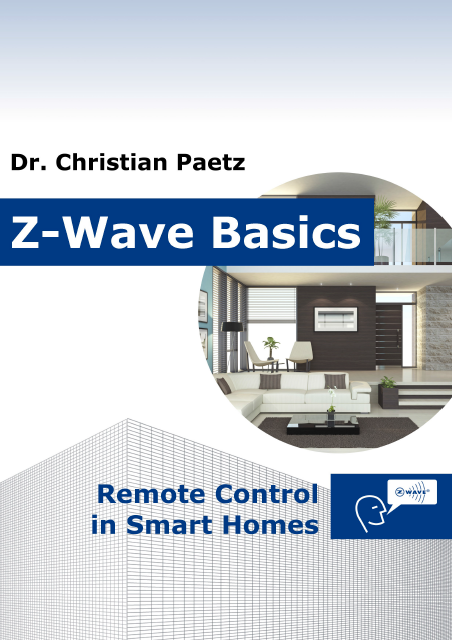
\includegraphics[scale=0.3]{pics/book.png}
\caption{Dr. Christian Paetz: Z-Wave Basics}
\label{c2:demorouting} 
\end{center} 
\end{figure}

\begin{figure} 
\begin{center}
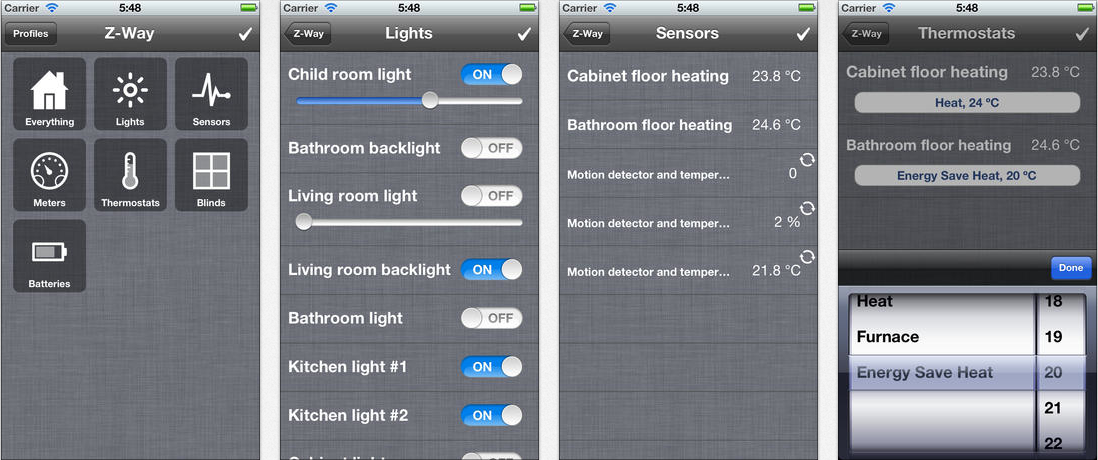
\includegraphics[scale=0.3]{pics/ipad.png}
\caption{iPhone/iPad App for Z-Way}
\label{c2:demorouting} 
\end{center} 
\end{figure}

\subsection{Mini Web UI}

The Mini UI Limited to about 800 lines of code this AJAX interface is a condensed version of the blue UI. 
It is a good starting point for writing AJAX based User Interfaces for RaZberry. You can download the most 
recent version of the mini UI free of charge from Github \footnote {https://github.com/PoltoS/z-way-mini-ui/}.

